\section{Filterschaltung}
In diesem Kapitel werden die Filterschaltungen zum splitten des Frequenzbereiches des Eingangssignals geplant, simuliert und gebaut.

\subsection{Methoden}
Das Teilen des Eingangssignals in zwei Frequenzbereiche lässt sich mit einem Hoch- und einem Tiefpass realisieren. Wichtig ist hierbei, dass beide Filter die Gleiche Grenzfrequenz besitzen, damit keine Frequenzen 'verloren gehen'. 1kHz ist eine sinnvolle Grenzfrequenz, da diese Frequenz in der logarithmischen Mitte zwischen 200Hz und 5000Hz liegt. Diese Werte entsprechen dem Frequenzintervall des Hauptsprachbereichs welche sich dem Diagramm\cite{Hoerbereichdiagramm} der Aufgabenstellung entnehmen lassen. \\
Des weiteren müssen beide Filter das Eingangssignal um den Faktor 1 verstärken und von 2ter Ordnung sein. Dies lässt sich mit, nach ihren Erfindern benannten, Sallen-Key Filtern erreichen.
Diese Annahme bezogen wir aus dem LEN-Skript.\\
Um eine Verstärkung von 1 zu erzielen bedarf es einer direkten Rückkopplung des Ausgangssignals auf den invertierenden Eingang des OpAmps. Die Schaltung im Computerprogramm LTSpice gebaut ist in folgender Abbildung zu sehen:

\begin{figure}[h]
	\centering
	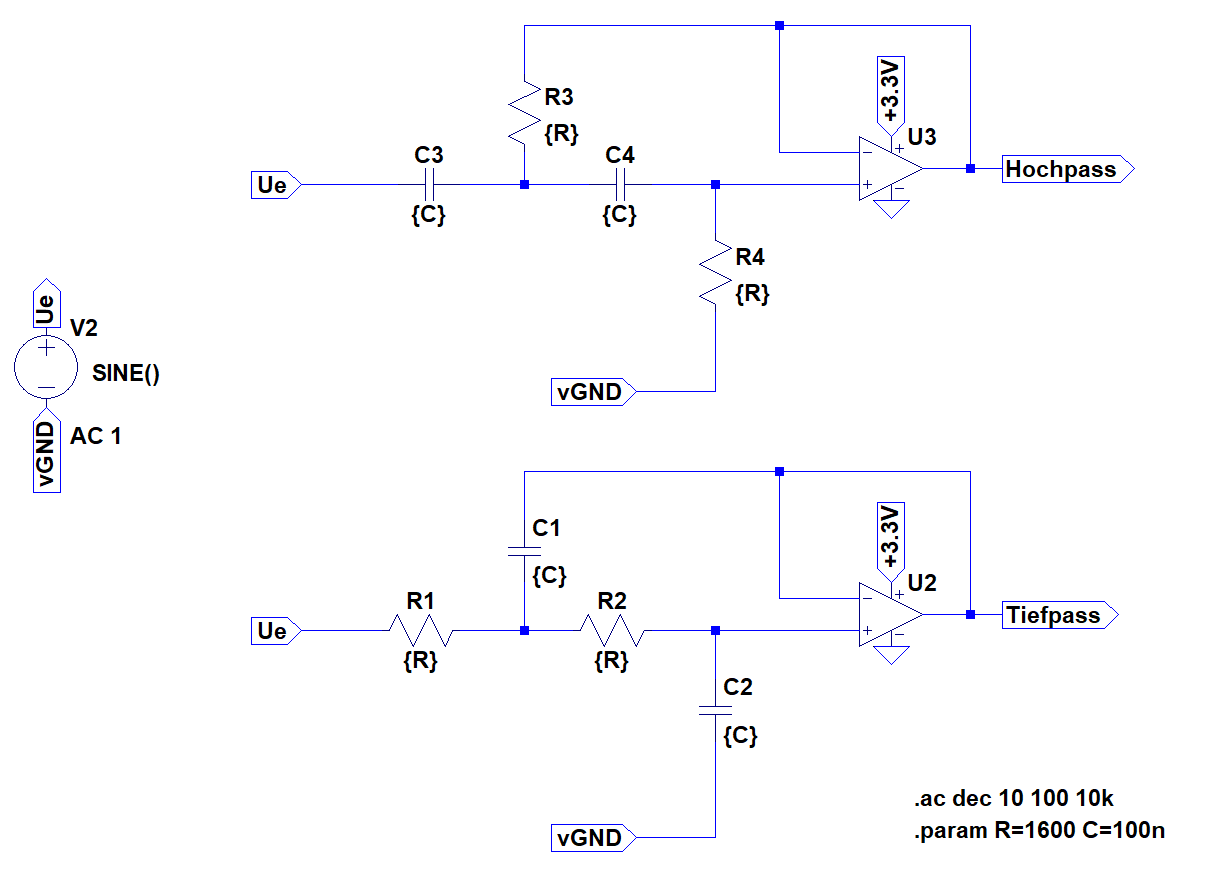
\includegraphics[width=1\textwidth]{pics/SpiceSchaltungFilter.PNG}
	\caption{Aufbau Hoch- und Tiefpass in LTSpice}
\end{figure}

Im folgenden werden die Werte für die Widerstände und die Kondensatoren bestimmt.
Für die Güte des Tiefpass-Filter gilt:

$$ Q = \frac{1}{2}\cdot\sqrt{\frac{C_{1}}{C_{2}}} $$

Die Anforderungen an die Filter verlangen eine Güte von 0,5. Daher gilt $C_{1}=C_{2}$.\\
Für $\omega_{0}$ beim Tiefpass ist gegeben:

$$\omega_{0}=\frac{1}{R\cdot\sqrt{C_{1} \cdot C_{2}}}$$

Da $C_{1}$ und $C_{2}$ den gleichen Wert haben sollen und die Grenzfrequenz $f_{0}=1\si{\kilo\hertz}$ betragen soll, ergibt sich:

$$\omega_{0}=2\pi f_{0} \approx 6283\si{\hertz} \, \Leftrightarrow \,\omega_{0}=\frac{1}{R\cdot C}\approx 6283\si{\hertz} $$

Da die uns zur Verfügung stehende Anzahl and verschiedenen Widerständen größer ist als die der Kondensatoren, haben wir $C_{1}=C_{2}=100\si{\nano\farad}$ gewählt.
Daraus ergibt sich $R=1592\si{\ohm}$. Damit erfüllt der Tiefpass-Filter alle geforderten Eigenschaften. \\
Für die Güte des Hochpass-Filter gilt:

$$Q=\frac{1}{2}\cdot\sqrt{\frac{R_{1}}{R_{2}}}$$

Es muss $R_{1}=R_{2}$ gewählt werden um auch beim Hochpass eine Güte von 0,5 zu bekommen.
Für $\omega_{0}$ ist gegeben:

$$\omega_{0} = \frac{1}{C\cdot\sqrt{R_{1}\cdot R_{2}}}$$

Aus $R_{1}=R_{2}$ folgt:

$$\omega_{0} = \frac{1}{C\cdot R}=6283\si{\hertz}$$

wir erhalten also die selbe Gleichung für die Eigenfrequenz wie beim vorher besprochenen Tiefpass-Filter. Wenn in beiden Filtern jeweils alle Kondensatoren und alle Widerstände den gleichen Wert haben, bekommen wir bei beiden Filtern die selbe Grenzfrequenz. Selbstverständlich ist möglich beim Tiefpass-Filter andere Werte zu nehmen als beim Hochpass-Filter. So lange man jedoch $C_{1}=C_{2}$ und $R_{1}=R_{2}$ gilt, weisen die Filter immer exakt das selbe Verhalten auf.\\
Wie schon erwähnt entscheiden wir uns für $C=100\si{\nano\farad}$, auf Grund der uns zur Verfügung stehenden Kondensatoren. Da sich ein exaktes $R=6283\si{\ohm}$ mit unseren Möglichkeiten nicht realisieren lässt, bauen wir die Filter mit einem 1500\si{\ohm} und einem 100\si{\ohm} Widerstand in Reihe geschaltet und erhalten so $R=1600\si{\ohm}$.\\
Somit gilt für unsere Grenzfrequenz:

$$\omega_{0}=\frac{1}{1600\si{\ohm}\cdot 100\si{\nano\farad}}=6250\si{\hertz}\Rightarrow f_{0}=\frac{\omega_{0}}{2\pi}\approx 995\si{\hertz}$$

Diese kleinen Abweichung von unseren angedachten 1\si{\kilo\hertz} macht nichts weiter aus, da wir trotzdem bei beiden Filtern die selbe Grenzfrequenz erhalten.
Somit entspricht die Schaltung allen Anforderungen der Aufgabenstellung.\\

Durch gezieltes auswählen der Maschen erhalten wir folgende Maschengleichungen:

$$M1:U_{e}=$$


\subsection{Ergebnisse}

\subsection{Diskussion}


